% -*- TeX -*-
%
% ----------------------------------------------------------------------
%
%                           Brad T. Aagaard
%                        U.S. Geological Survey
%
% {LicenseText}
%
% ----------------------------------------------------------------------
%
\documentclass[pdftex,cig,slideColor]{pp4slides}
\usepackage{amsmath}
\usepackage{array}
\usepackage{xspace}
\usepackage{multirow}
\usepackage{ulem}

\newcommand{\newfeature}[1]{{\color{blue}#1}}

\title{Extending PyLith}
\author{Brad Aagaard and Charles Williams\\[10pt]
  Matthew Knepley and Surendra Somala}
\institution{\includegraphics[height=2cm]{../../logos/cig}}
\date{June 15, 2010}

% --------------------------------------------------------- DOCUMENT
\begin{document}

% ------------------------------------------------------------ SLIDE
\maketitle

% ------------------------------------------------------------ SLIDE
\foilhead{How can PyLith be extended?}
  \summary{}

  \begin{itemize}
  \item Any component can be replaced
    \begin{itemize}
    \item Custom spatial databases
    \item Bulk constitutive models
    \item Fault constitutive models
    \item Solvers
    \item Boundary conditions
    \end{itemize}
  \item Difficult to change: governing equations
    \begin{itemize}
    \item Coupled fluid flow
    \item Coupled heat flow
    \end{itemize}
  \end{itemize}  


\bgadd{\vspace*{7.9in}%
  \begin{center}%
    \includegraphics[height=14mm]{../../logos/cig}
  \end{center}}


% ------------------------------------------------------------ SLIDE
\foilhead{Prerequisites for Adding Components}
  \summary{Recommended for advanced users only}

  \begin{itemize}
  \item Comfortable working with
    \begin{itemize}
    \item Makefiles
    \item Python
    \item C/C++
    \item Object-oriented programming
    \end{itemize}
  \item Good at pattern matching
  \item Desire to break new ground
  \end{itemize}    


% ------------------------------------------------------------ SLIDE
\foilhead{Anatomy of a PyLith Component}
  \summary{}

  \vfill
  \begin{center}
    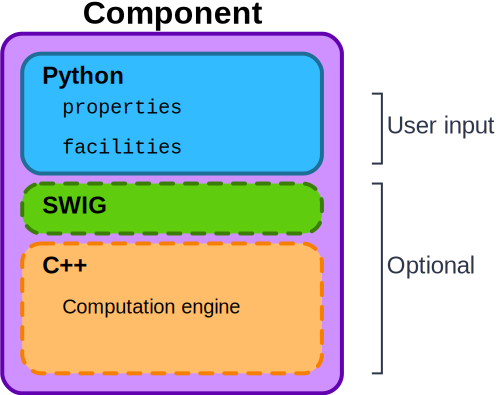
\includegraphics[scale=1.0]{figs/component}
  \end{center}  
  \vfill


% ------------------------------------------------------------ SLIDE
\foilhead{Implementation of a PyLith Component}
  \summary{}

  \begin{itemize}
  \item Python object
    \begin{itemize}
    \item Gather user input
    \item Do high-level validation of parameters
    \item Send user input to C++
    \end{itemize}
  \item C++ object
    \begin{itemize}
    \item Accept user input from Python
    \item Implement interface required for component
    \end{itemize}
  \end{itemize}


% ------------------------------------------------------------ SLIDE
\foilhead{Example: Bulk Constitutive Model}
  \summary{Elastic plane strain w/state variables}

  \begin{itemize}
  \item Python object
    \begin{itemize}
    \item User defined parameters: none
    \item Inherited from Elastic material
      \begin{itemize}
      \item {\tt db\_properties}
      \item {\tt db\_initial\_state}
      \end{itemize}
    \end{itemize}
  \item C++ object
    \begin{itemize}
    \item Define physical properties and state variables
    \item Convert db parameters to values used internally
    \item Nondimensionalization of parameters
    \item Implement rheology \\
      Calculate density, stresses, and elastic constants
    \end{itemize}
  \item Verify functionality using unit tests
  \end{itemize}
 
 

 
% ======================================================================
\end{document}


% End of file
